\documentclass[11pt]{article}
\usepackage[margin=1in]{geometry}
\usepackage{graphicx,booktabs,hyperref,float}
\graphicspath{{figures/}}
\title{Assignment 3: Federated Learning and Differential Privacy}
\author{GitHub: \texttt{aasritha-oql7872} \quad Repository: \texttt{mlds-assignment3}\\
\url{https://github.com/aasritha-oql7872/mlds-assignment3}}
\date{}
\begin{document}\maketitle

\section*{Running the code (deepdish)}
\begin{verbatim}
git clone https://github.com/aasritha-oql7872/mlds-assignment3.git
cd mlds-assignment3
python3 -m venv ~/fl_env && source ~/fl_env/bin/activate
pip install -r requirements.txt
export CUDA_VISIBLE_DEVICES=<idle gpu>       # one GPU max
# place train_data.npy and test_data.npy in ./data
python validation_tests.py --data data       # 11 validation checks
bash experiments.sh data                     # all sweeps -> results/*.json
python plots.py --data data                  # all figures -> figures/
\end{verbatim}
Single runs: \texttt{python run.py --data data --C 0.1 --E 10 [--parallel] [--b 0.1]}.
Files: \texttt{fl.py} (data, model, Ray actor, FedAvg), \texttt{run.py}, \texttt{experiments.sh}, \texttt{plots.py}, \texttt{validation\_tests.py}.\sloppy

\section*{Setup common to both parts}
Model: 784--128--62 MLP with ReLU. Each client's data is split 80\%/20\% into train/validation; the provided held-out \texttt{test\_data.npy} (3621 images) is used only for the final test accuracy and is never perturbed. FedAvg is written from scratch: the server samples $\lceil C\cdot 100\rceil$ clients per round, each runs $E$ epochs of SGD (batch 32) from the current global weights, and the server sets the global weights to the $n_k$-weighted mean of the returned weights ($n_k$ = number of local training samples). Reported train/validation loss and accuracy are of the \emph{global} model evaluated on the union of all clients' train/validation data after each round. Learning rate and rounds were tuned on validation accuracy: $\mathrm{lr}\ge 0.1$ diverged on this non-IID data (test acc.\ 0.18 at lr 0.1, 0.06 at lr 0.2, $E{=}5$), so lr $=0.03$, 500 rounds were used everywhere (seed 0).

\section{Part 1: FedAvg on Federated EMNIST}
\subsection*{1.1 Data distribution}
There are 100 clients, 31{,}825 training images (118--393 per client). Classes are heavily imbalanced overall (56 to 1837 images per class; class 40, lowercase ``e'', is the largest; 30\% digits, 39\% uppercase, 31\% lowercase) and each client sees only about 55 of the 62 classes, with a client-specific mix (Fig.~\ref{fig:dist}); the five sampled users (26, 86, 2, 55, 75) have 275--354 images, 53--59 classes, and their most frequent class (class 40 for all five) makes up only 8--15\% of their data. The data is therefore non-IID in label proportions (and in writer style), which is why local training drifts and large learning rates fail.
\begin{figure}[H]\centering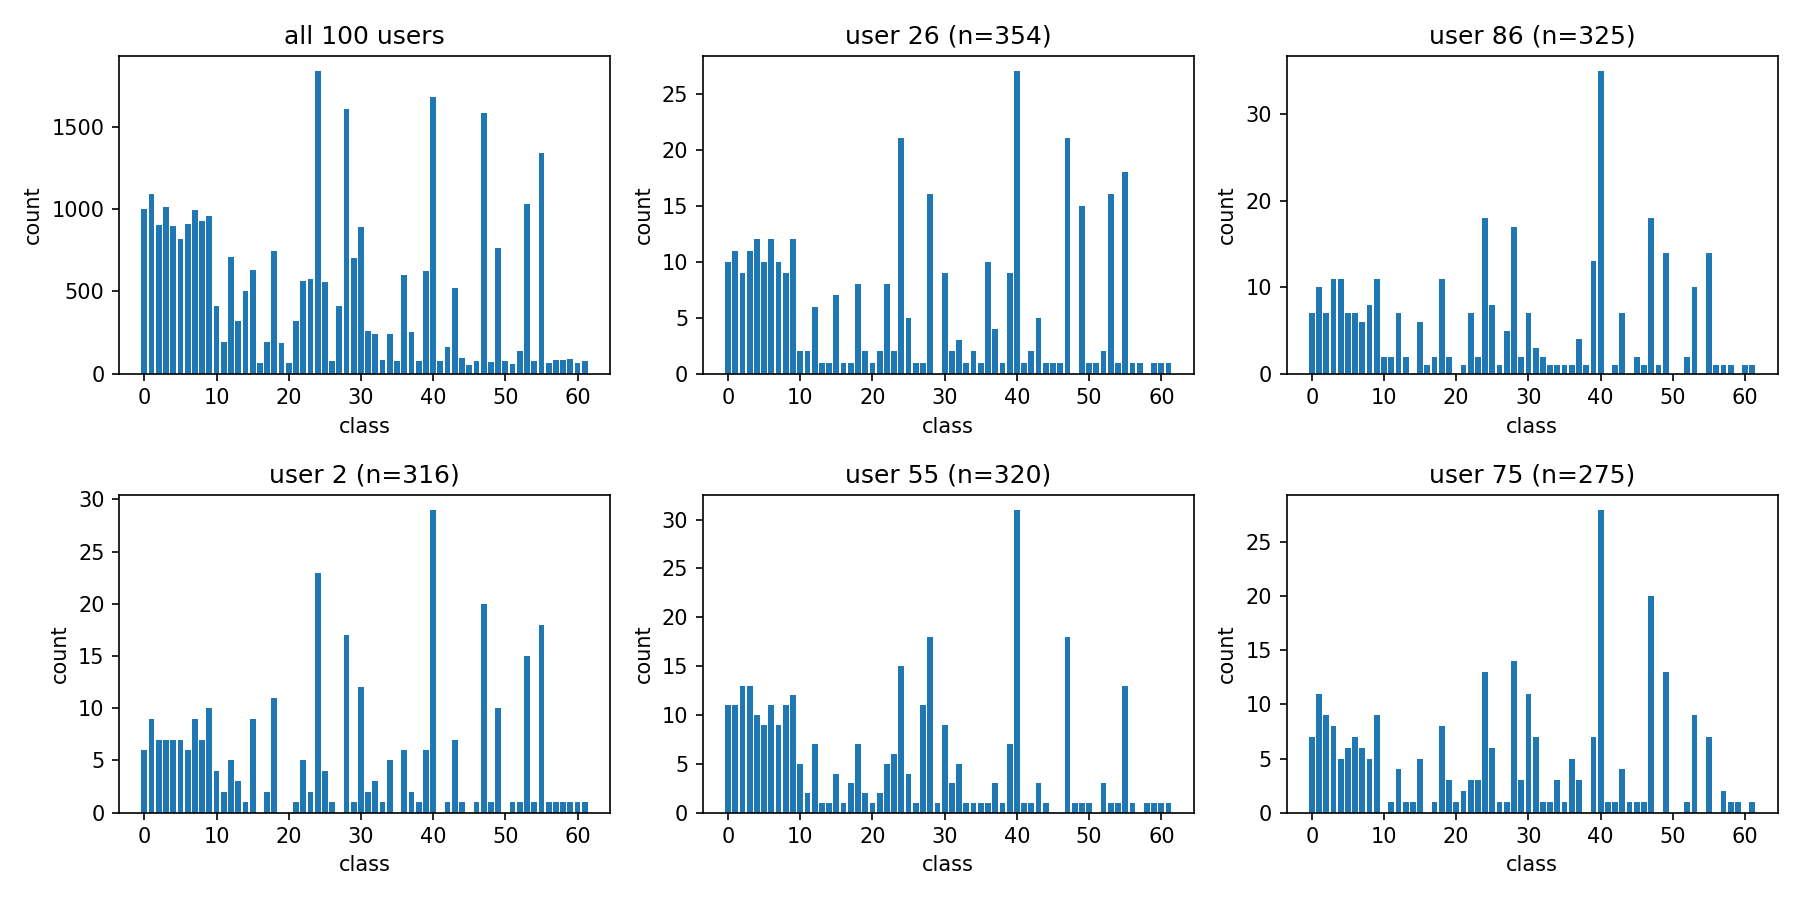
\includegraphics[width=.9\linewidth]{data_distribution}\caption{Class counts: all clients (top left) and 5 users.}\label{fig:dist}\end{figure}

\subsection*{1.2--1.4 Training curves and effect of $C$ and $E$}
\begin{figure}[H]\centering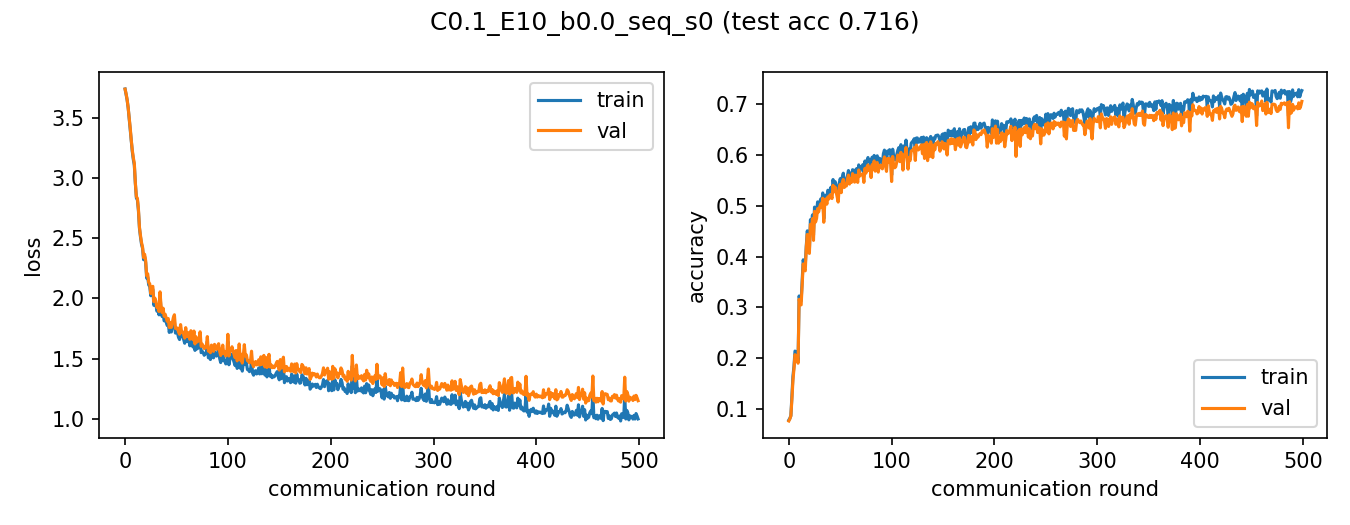
\includegraphics[width=.9\linewidth]{C0.1_E10_b0.0_seq_s0}\caption{Train/validation loss and accuracy vs.\ rounds, $C{=}0.1$, $E{=}10$ (best configuration).}\end{figure}
\begin{table}[H]\centering\begin{tabular}{llccc}\toprule $C$ & $E$ & train acc & val acc & test acc\\\midrule
0.02 & 1 & 0.397 & 0.394 & 0.406\\0.02 & 5 & 0.606 & 0.597 & 0.595\\0.02 & 10 & 0.600 & 0.580 & 0.587\\
0.05 & 1 & 0.558 & 0.547 & 0.563\\0.05 & 5 & 0.681 & 0.663 & 0.669\\0.05 & 10 & 0.686 & 0.669 & 0.675\\
0.1 & 1 & 0.562 & 0.550 & 0.559\\0.1 & 5 & 0.691 & 0.674 & 0.681\\\textbf{0.1} & \textbf{10} & \textbf{0.727} & \textbf{0.706} & \textbf{0.716}\\\bottomrule\end{tabular}\caption{Final accuracy after 500 rounds (C $\le$ 10\% as required).}\end{table}
\begin{figure}[H]\centering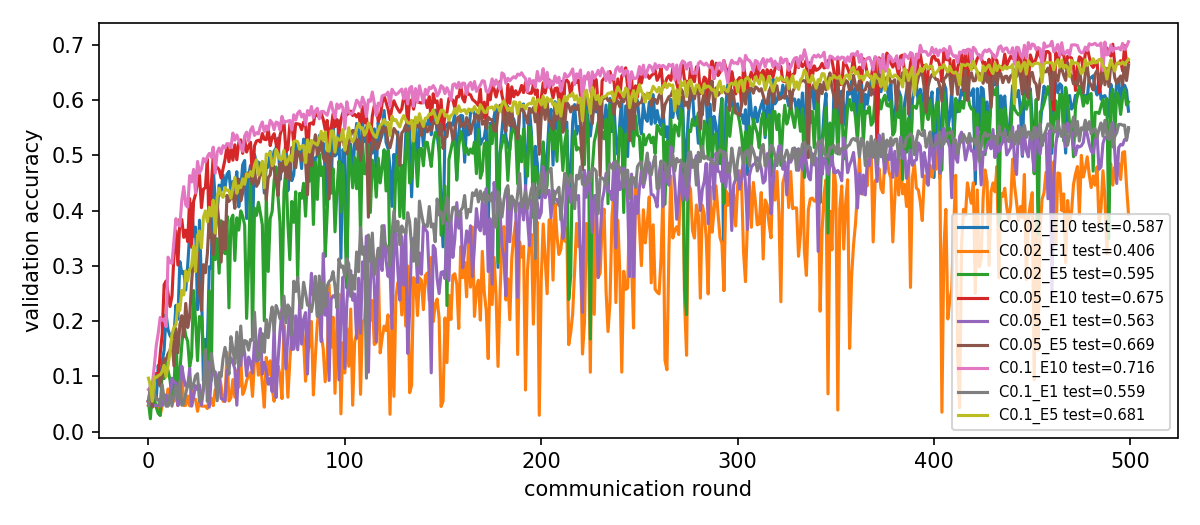
\includegraphics[width=.8\linewidth]{part1_C_E}\caption{Validation accuracy vs.\ round for all $(C,E)$.}\end{figure}
More local epochs and more clients per round both help: $E{=}1\to 10$ raises test accuracy by 11--18 points at every $C$, but $E{=}5$ and $E{=}10$ are nearly equal for $C\le 0.05$ (extra local epochs on few clients mostly fit those clients' own distributions), whereas at $C{=}0.1$ the gain continues (0.681 $\to$ 0.716). Larger $C$ averages more clients, reducing the variance of the update, so curves are smoother and higher. \textbf{Chosen hyperparameters: $C=0.1$, $E=10$, lr $0.03$, batch 32, 500 rounds; test accuracy $=0.716$.} Train and validation are close (0.727 vs.\ 0.706), so there is little overfitting; the validation curve is still creeping upward at round 500.

\subsection*{1.5 Parallel clients with Ray}
Each selected client is a Ray \texttt{Actor} (\texttt{num\_cpus=1}, optional \texttt{--gpus} fraction $\le 1$) created only for the 4 clients sampled in that round and killed afterwards; only the global weights go to the actor and only updated weights return. With 4 clients/round ($C{=}0.04$), $E{=}10$: train 0.664, validation 0.642, \textbf{test 0.658}. This is lower than $C{=}0.1$ for the reason above (fewer clients per round), and consistent with the sequential $C{=}0.05$ result (0.675).
\begin{figure}[H]\centering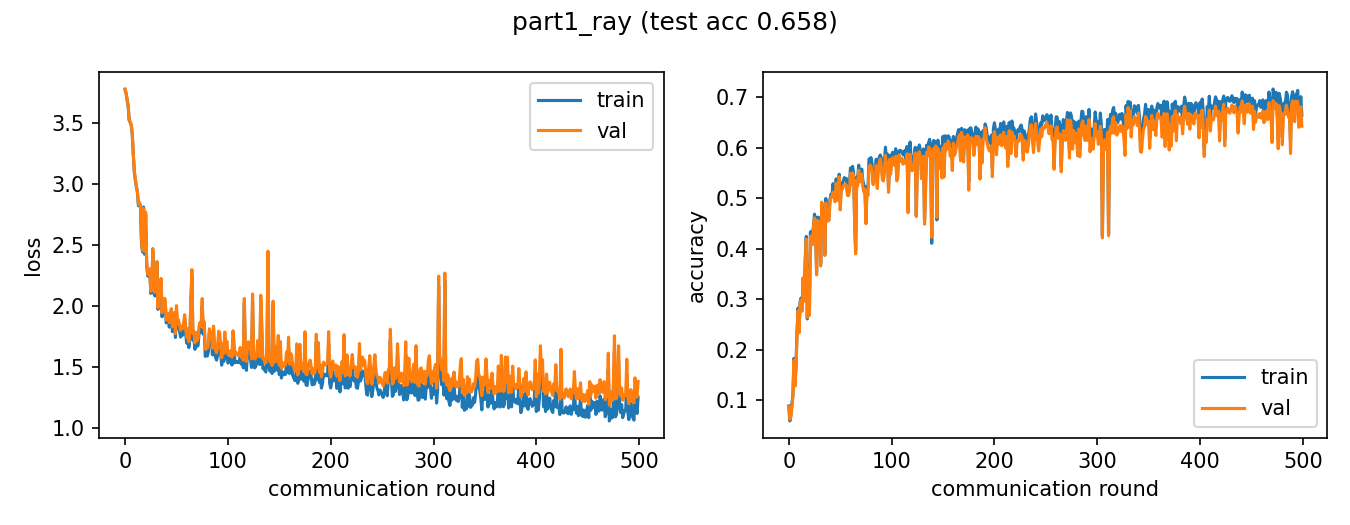
\includegraphics[width=.9\linewidth]{part1_ray}\caption{Ray run, 4 clients per round.}\end{figure}

\section{Part 2: Laplace mechanism}
Each train and validation image gets i.i.d.\ Laplace$(0,b)$ noise added once, before training (the test set is clean; pixels are in $[0,1]$). Settings are those chosen in Part 1 ($C{=}0.1,E{=}10$). Fig.~\ref{fig:b02} shows the curves for $b{=}0.2$.
\begin{figure}[H]\centering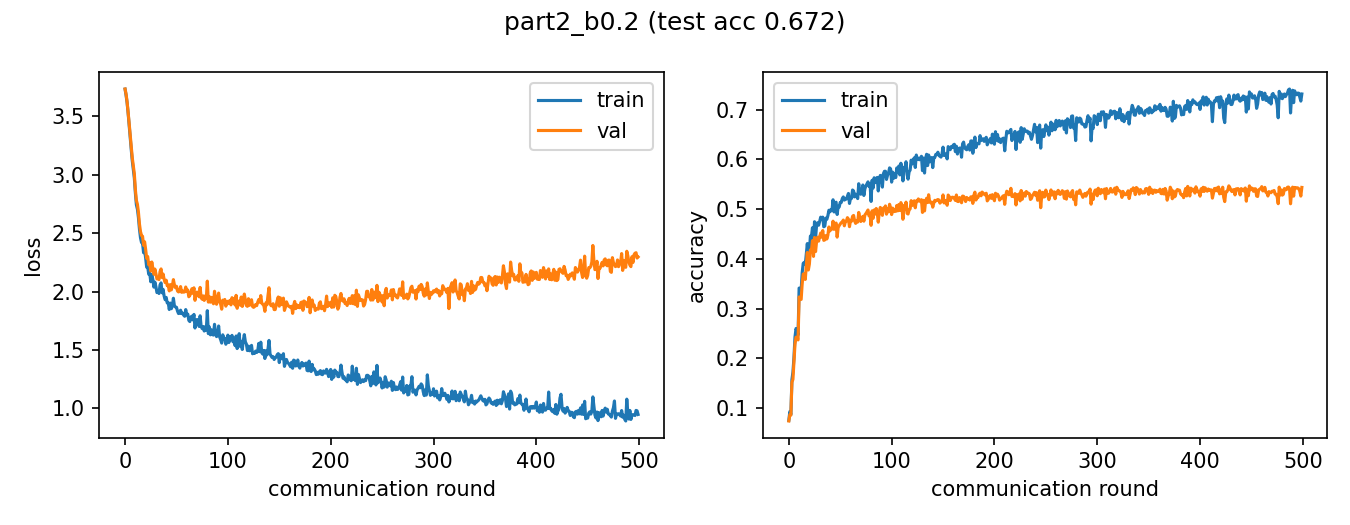
\includegraphics[width=.9\linewidth]{part2_b0.2}\caption{Training/validation loss and accuracy vs.\ rounds with $b=0.2$.}\label{fig:b02}\end{figure}
\begin{table}[H]\centering\begin{tabular}{lcccccccc}\toprule $b$ & 0 & 0.05 & 0.1 & 0.2 & 0.5 & 1.0 & 2.0\\\midrule
train acc & 0.727 & 0.735 & 0.737 & 0.731 & 0.654 & 0.727 & 0.835\\
val acc & 0.706 & 0.696 & 0.667 & 0.544 & 0.222 & 0.081 & 0.044\\
test acc & 0.716 & 0.712 & 0.707 & 0.672 & 0.534 & 0.317 & 0.103\\\bottomrule\end{tabular}\end{table}
\begin{figure}[H]\centering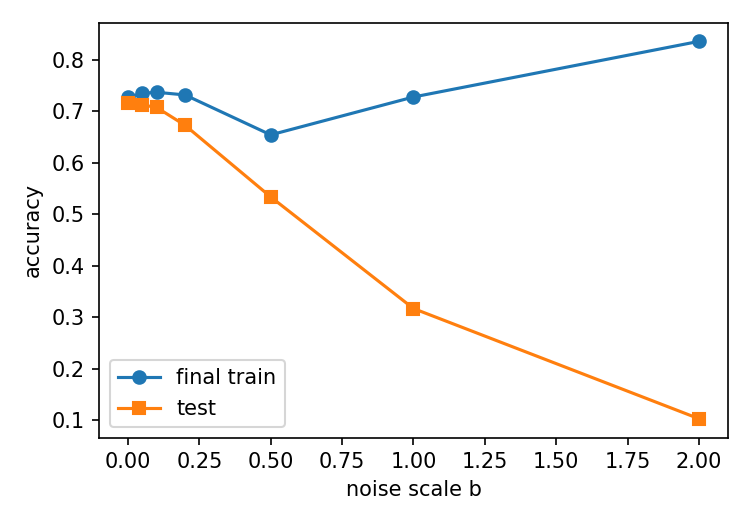
\includegraphics[width=.55\linewidth]{part2_noise}\caption{Final train and test accuracy vs.\ noise scale $b$.}\end{figure}
\textbf{Discussion.} Test accuracy decreases monotonically with $b$: negligible loss up to $b{=}0.1$ ($-0.9$ pts), moderate at $0.2$ ($-4.4$), severe at $0.5$ ($-18$) and near chance (1.6\%) at $b{=}2$ (0.103). Training accuracy does \emph{not} decrease: because the noise is drawn once, the MLP can memorise each client's fixed noisy images (train 0.835 at $b{=}2$) while generalising to nothing; the independently-noised validation set and the clean test set expose this, so the train--test gap, not train accuracy, measures the damage. I would use $\mathbf{b=0.1}$: it keeps test accuracy within one point of the noise-free model while still adding per-pixel noise of mean magnitude 0.1 (10\% of the pixel range); $b{=}0.2$ is the largest value that still keeps accuracy above 0.67. Caveat: this per-pixel noise gives no strong formal guarantee --- the $\ell_1$ sensitivity of an image with pixels in $[0,1]$ is up to 784, so $b{=}0.1$ corresponds to $\varepsilon\approx 784/0.1$ for replacing an entire image; the privacy it offers is empirical (obscuring pixels), not a meaningful $\varepsilon$-DP bound.

\section{Edge cases, validation tests, and non-standard plot}
\subsection*{Edge cases considered}
\begin{itemize}
\item \emph{Non-IID, unbalanced clients (118--393 samples)}: averaging must be weighted by $n_k$, not $1/K$; verified by test 3.
\item \emph{Clients re-sampled / not sampled}: sampling is without replacement within a round; every client can recur across rounds (heatmap).
\item \emph{Test leakage}: test set is a separate file, never noised or trained on; test 6 checks no test image appears in client data. Noise is added to train/validation only.
\item \emph{Noise changing the split or labels}: noise uses its own RNG, so splits and labels are identical with and without noise (test 5), making runs with different $b$ comparable.
\item \emph{Ray determinism and memory}: actors are created only for selected clients and killed each round; per-client seeds are drawn on the server so Ray and sequential runs are comparable (test 4).
\item \emph{Divergence}: large learning rates diverge under non-IID updates; found by sweeping lr, and the threshold is documented above.
\item \emph{Tiny/empty splits}: validation size is $\max(1,\lfloor 0.2n\rfloor)$; the smallest client has 118 samples so no split is empty.
\end{itemize}
\subsection*{Validation tests (\texttt{python validation\_tests.py --data data}; all 11 pass on deepdish)}
\begin{enumerate}
\item \textbf{Single client = plain SGD.} FedAvg with one client reproduces local training exactly (max weight diff $<10^{-6}$): checks the server/aggregation plumbing.
\item \textbf{$E{=}0$.} With zero local epochs the global model stays at its initialisation: no hidden state changes.
\item \textbf{Weighted aggregation.} For the largest and smallest clients (weights 0.768/0.232) the global model equals the hand-computed $n_k$-weighted mean.
\item \textbf{Ray $=$ sequential.} Same seed gives the same model (max diff $2.2\times10^{-8}$ on deepdish).
\item \textbf{Noise statistics.} Mean $|\varepsilon|$ for $b{=}0.5$ is 0.500 (Laplace$(b)$ has $E|\varepsilon|=b$); labels unchanged.
\item \textbf{Partition / no leakage.} Train+val sizes equal client sizes; test images do not occur in client data.
\item \textbf{Behaviour.} After 30 rounds test accuracy is 0.176 vs.\ 0.022 for a random init ($\approx 1/62$); with $b{=}50$ it falls to 0.028.
\item \textbf{More local epochs lowers local loss} ($E{=}1\to10$: 1036 $\to$ 992).
\end{enumerate}
Beyond these: the $C$/$E$ sweep (more clients or epochs $\Rightarrow$ better) and the noise sweep (monotone test-accuracy decay, train/test gap growing with $b$) match theory.

\subsection*{Non-standard plot: client participation heatmap}
Rows are the 100 clients, columns are rounds, and colour is the selected client's local validation accuracy after its local update (blank = not selected). Early rounds show many poor local models (dark); they brighten as the global model improves, and no row is visibly empty or consistently dark, consistent with random 10\% sampling covering all clients.
\begin{figure}[H]\centering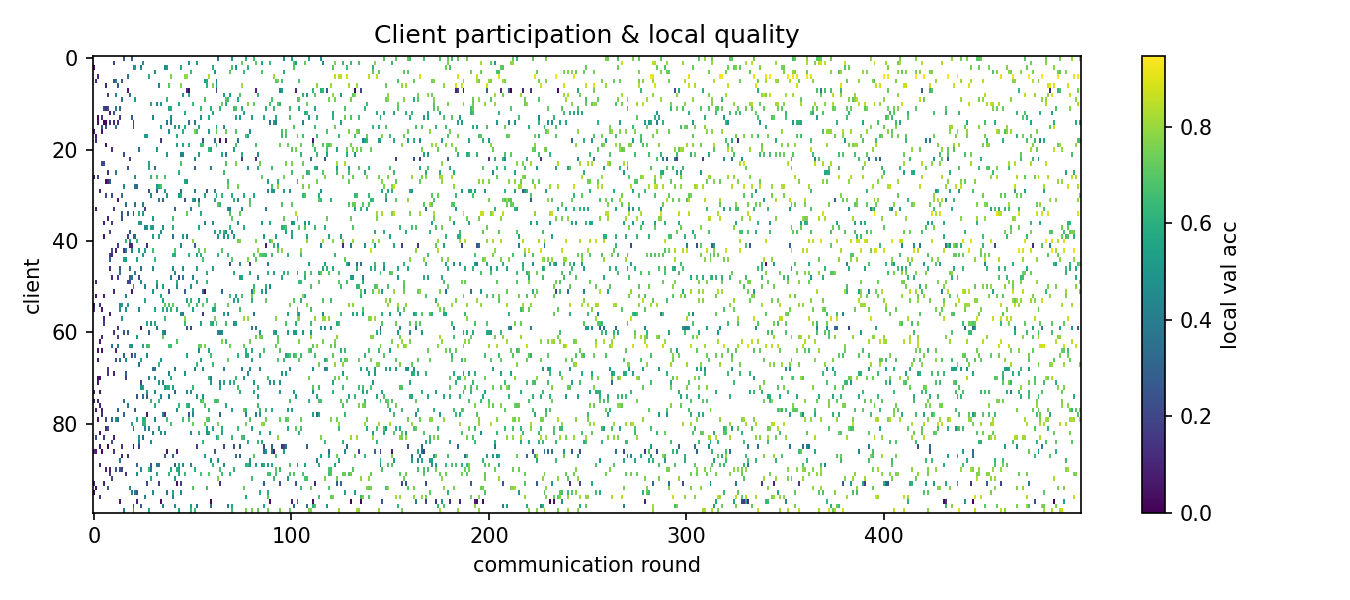
\includegraphics[width=.9\linewidth]{participation_heatmap}\caption{Client participation and local accuracy ($C{=}0.1$, $E{=}10$).}\end{figure}

\section{With an additional 3 months, what else would I test?}
\begin{itemize}
\item Multiple seeds (e.g.\ 10) with confidence intervals for every table entry, so that differences like 0.675 vs.\ 0.669 can be called significant.
\item Fresh noise each epoch/round vs.\ a fixed noise draw, to separate memorisation of noise from true noise robustness.
\item Real differential privacy: clipping per-example gradients with Gaussian/Laplace noise (DP-SGD / DP-FedAvg), a privacy accountant for $(\varepsilon,\delta)$, and membership-inference/reconstruction attacks to check that empirical leakage falls as the noise grows.
\item FedProx/SCAFFOLD/server momentum against FedAvg to test whether client drift is the bottleneck; learning-rate decay; per-client accuracy to measure fairness across writers.
\item Straggler and dropout simulation (clients failing mid-round), and non-uniform sampling by $n_k$.
\item Convergence to the centralised-training upper bound, and scaling Ray to more clients/GPUs with timing.
\end{itemize}
\end{document}
